% Rapport de projet — SUVAC
% Module Développement Web Backend — Master 1 MILIA
% École Polytechnique de Thiès, 2026-2027
%
% Compilation : pdflatex rapport.tex (deux fois pour la table des matières)
%
% Arborescence attendue :
%   rapport.tex
%   images/logo-ept.png
%   images/architecture.png
%   uml/01-cas-utilisation.png ... uml/07-deploiement.png
%   captures/01-connexion.png ... captures/12-whatsapp-recu.jpg

\documentclass[11pt,a4paper]{report}

\usepackage[utf8]{inputenc}
\usepackage[T1]{fontenc}
\usepackage[french]{babel}
\usepackage{lmodern}
\usepackage{microtype}

\usepackage[margin=2.5cm]{geometry}
\usepackage{graphicx}
\usepackage{float}
\usepackage{booktabs}
\usepackage{tabularx}
\usepackage{longtable}
\usepackage{xcolor}
\usepackage{fancyhdr}
\usepackage{titlesec}
\usepackage{enumitem}
\usepackage{listings}
\usepackage{caption}
\usepackage[hidelinks]{hyperref}

% --- Couleurs sobres, lisibles à l'impression ----------------------
\definecolor{accent}{HTML}{1F4E3D}
\definecolor{gris}{HTML}{555555}
\definecolor{grisclair}{HTML}{F4F4F4}

% --- En-têtes et pieds de page -------------------------------------
\pagestyle{fancy}
\fancyhf{}
\fancyhead[L]{\small\textcolor{gris}{SUVAC — Suivi vaccinal et rappels vocaux en wolof}}
\fancyfoot[C]{\small\thepage}
\renewcommand{\headrulewidth}{0.4pt}

% --- Titres ---------------------------------------------------------
\titleformat{\chapter}[display]
  {\normalfont\huge\bfseries\color{accent}}
  {\chaptertitlename\ \thechapter}{10pt}{\Huge}
\titlespacing*{\chapter}{0pt}{-20pt}{30pt}

\titleformat{\section}
  {\normalfont\Large\bfseries\color{accent}}{\thesection}{1em}{}

% --- Code -----------------------------------------------------------
\lstset{
  basicstyle=\ttfamily\footnotesize,
  backgroundcolor=\color{grisclair},
  frame=single,
  rulecolor=\color{gris},
  breaklines=true,
  captionpos=b,
  showstringspaces=false,
  literate=
    {é}{{\'e}}1 {è}{{\`e}}1 {ê}{{\^e}}1 {ë}{{\"e}}1
    {à}{{\`a}}1 {â}{{\^a}}1 {ç}{{\c c}}1
    {ô}{{\^o}}1 {ö}{{\"o}}1 {î}{{\^i}}1 {ï}{{\"i}}1
    {û}{{\^u}}1 {ù}{{\`u}}1 {ü}{{\"u}}1
    {ñ}{{\~n}}1 {Ñ}{{\~N}}1
    {É}{{\'E}}1 {È}{{\`E}}1 {À}{{\`A}}1 {Ç}{{\c C}}1
}

% --- Légendes -------------------------------------------------------
\captionsetup{font=small, labelfont={bf,color=accent}}

% --- Raccourcis ------------------------------------------------------
\newcommand{\capture}[3]{%
  \begin{figure}[H]
    \centering
    \includegraphics[width=#2\textwidth]{captures/#1}
    \caption{#3}
  \end{figure}
}

\newcommand{\diagramme}[3]{%
  \begin{figure}[H]
    \centering
    \includegraphics[width=#2\textwidth, height=0.80\textheight, keepaspectratio]{uml/#1}
    \caption{#3}
  \end{figure}
}

\begin{document}

% ====================================================================
% PAGE DE GARDE
% ====================================================================
\begin{titlepage}
\centering


\includegraphics[width=0.28\textwidth]{images/logo-ept.png}

\vspace{0.8cm}

{\large\textbf{ÉCOLE POLYTECHNIQUE DE THIÈS}}\\[0.3cm]
{\normalsize Département Génie Informatique et Télécommunications}\\[1.2cm]

{\normalsize Master Ingénierie Logicielle et Intelligence Artificielle}\\[0.2cm]
{\normalsize Première année}\\[1.5cm]

\rule{\textwidth}{1.2pt}\\[0.6cm]

{\LARGE\bfseries\color{accent} SUVAC — Kaay Ñakku}\\[0.5cm]

{\large Plateforme de suivi de la vaccination pré et post natale\\
avec rappels vocaux en wolof}\\[0.6cm]

\rule{\textwidth}{1.2pt}\\[1.5cm]

{\normalsize\textbf{Module} : Développement Web Backend}\\[2cm]

\begin{minipage}{0.45\textwidth}
  \begin{flushleft}
    \textbf{Réalisé par :}\\[0.2cm]
    Fallou DIOUCK
  \end{flushleft}
\end{minipage}
\hfill
\begin{minipage}{0.45\textwidth}
  \begin{flushright}
    \textbf{Encadré par :}\\[0.2cm]
    Professeur Michel SECK
  \end{flushright}
\end{minipage}

\vspace{2cm}

{\small Code source :\\
\url{https://github.com/Fallou236/suvac}}

\vfill

{\normalsize Année universitaire 2026 — 2027}

\end{titlepage}

% ====================================================================
% RÉSUMÉ
% ====================================================================
\chapter*{Résumé}
\addcontentsline{toc}{chapter}{Résumé}

SUVAC est une plateforme web de suivi de la vaccination pré et post natale
conçue pour les postes de santé sénégalais. Elle calcule le calendrier
vaccinal de chaque bénéficiaire à partir du schéma du Programme Élargi de
Vaccination, affiche à l'agent la file des personnes attendues chaque
matin, et envoie aux mères un rappel avant chaque échéance.

La particularité du système tient à la forme de ce rappel. Au Sénégal, une
part importante des femmes en âge de procréer ne lit pas couramment le
français. Un message écrit ne les atteint pas. SUVAC leur adresse donc un
\emph{message vocal en wolof}, synthétisé à partir du texte composé par le
système, encapsulé dans une vidéo et remis par WhatsApp.

Le travail a été mené en trois sprints sur un dépôt Git public, avec
intégration continue, tests automatisés et décisions d'architecture
documentées. Au terme du projet, 286 tests couvrent 87\% du code serveur et
l'interface atteint 85,6\% de couverture. La chaîne complète a été vérifiée
de bout en bout : un rappel vaccinal composé en wolof, prononcé par
synthèse vocale, est parvenu sur un téléphone sénégalais.

\bigskip
\noindent\textbf{Mots-clés} : santé maternelle et infantile, vaccination,
wolof, synthèse vocale, Django, React, WhatsApp Business API.

% ====================================================================
% TABLE DES MATIÈRES
% ====================================================================
\tableofcontents
\clearpage

% ====================================================================
% CHAPITRE 1 — INTRODUCTION
% ====================================================================
\chapter{Introduction}

\section{Contexte}

La vaccination infantile est l'une des interventions de santé publique au
meilleur rapport coût-efficacité. Au Sénégal, le Programme Élargi de
Vaccination définit un calendrier précis : neuf vaccins, administrés selon
des échéances calculées à partir de la date de naissance, certaines doses
devant respecter un intervalle minimal entre elles.

Ce calendrier est consigné dans un carnet papier remis à la mère. Ce carnet
présente deux faiblesses. Il se perd, et sa perte emporte avec elle
l'historique vaccinal de l'enfant. Surtout, il ne rappelle rien : c'est à la
mère de se souvenir de la date du prochain rendez-vous, souvent plusieurs
semaines à l'avance.

La conséquence est connue des agents de santé : l'abandon en cours de série.
Un enfant reçoit sa première dose de pentavalent, puis la deuxième n'est
jamais administrée. Les doses manquées ne sont pas détectées, parce que rien
ne signale l'absence — un bénéficiaire qui ne vient pas n'apparaît nulle
part.

\section{Problème}

Deux obstacles séparent le système de santé de la mère.

Le premier est celui de l'information : personne ne sait, un matin donné,
quels enfants devraient se présenter au poste. Le registre est une liste
chronologique des passages, pas un calendrier des échéances à venir.

Le second est celui de la langue. Les outils numériques de santé s'adressent
en français à une population dont une part importante ne le lit pas. Selon
les données de l'ANSD, le taux d'alphabétisation des femmes en milieu rural
reste nettement inférieur à celui des hommes, et le français n'est pas la
langue de la vie quotidienne dans la plupart des foyers. Un rappel par SMS
écrit en français n'atteint pas sa destinataire.

\section{Objectifs}

L'objectif général est de \textbf{réduire les doses manquées en rendant
visible ce qui est dû et en prévenant la bénéficiaire dans une langue
qu'elle comprend}.

Il se décline en quatre objectifs spécifiques :

\begin{enumerate}[label=\textbf{OS-\arabic*.}, leftmargin=1.5cm]
  \item Calculer et tenir à jour le calendrier vaccinal de chaque
  bénéficiaire à partir du schéma officiel, y compris après une dose
  manquée ou administrée hors délai.
  \item Donner à l'agent de santé une vue quotidienne des personnes
  attendues et de celles en retard.
  \item Prévenir les mères avant chaque échéance par un message vocal en
  wolof, acheminé par un canal qu'elles utilisent déjà.
  \item Donner au superviseur les indicateurs de couverture et
  d'acheminement nécessaires au pilotage de son poste.
\end{enumerate}

\section{Objectifs pédagogiques}

Au-delà du produit, le projet visait à mettre en œuvre les pratiques
enseignées dans le cursus : conception orientée objet avec UML, API REST
documentée, tests automatisés, intégration continue, et traçabilité des
décisions d'architecture.

\section{Périmètre}

\subsection*{Dans le périmètre}

Le suivi vaccinal des enfants de zéro à cinq ans et des femmes enceintes ;
le moteur de calendrier ; les rappels par WhatsApp et leur production
vocale ; un espace de consultation pour les mères ; le pilotage par poste ;
l'administration des comptes et des postes.

\subsection*{Hors périmètre}

La gestion des stocks de vaccins, la chaîne du froid, la facturation, et
l'interopérabilité avec le système national d'information sanitaire. Le mode
hors ligne, bien que spécifié, n'a pas été réalisé dans le temps imparti ; il
est traité au chapitre des perspectives.

\section{Méthode de travail}

Le développement a suivi un cycle itératif, proche du cycle en spirale : le
cahier des charges a été découpé en trois incréments fonctionnels, chacun
traité comme un sprint avec sa planification, sa réalisation et sa
rétrospective.

\begin{table}[H]
\centering
\begin{tabularx}{\textwidth}{@{}llX@{}}
\toprule
\textbf{Sprint} & \textbf{Thème} & \textbf{Contenu} \\
\midrule
S-1 & Socle métier & Modèle de données, moteur de calendrier, API REST,
cloisonnement par poste \\
S-2 & Interface & Application React, écrans de l'agent, tableau de bord du
superviseur, espace bénéficiaire \\
S-3 & Communication & Planification des rappels, composition wolof,
synthèse vocale, canal WhatsApp, administration \\
\bottomrule
\end{tabularx}
\caption{Découpage en sprints}
\end{table}

Chaque sprint a donné lieu à un avenant au cahier des charges, et les
décisions structurantes ont été consignées dans des fiches ADR
(\emph{Architecture Decision Records}) — neuf au total, référencées tout au
long de ce rapport.

% ====================================================================
% CHAPITRE 2 — ANALYSE DES BESOINS
% ====================================================================
\chapter{Analyse des besoins}

\section{Acteurs du système}

Conformément à la définition d'UML, un acteur correspond à un rôle et non à
une personne physique : la même personne peut être agent un jour et
superviseur un autre.

\begin{table}[H]
\centering
\begin{tabularx}{\textwidth}{@{}lXl@{}}
\toprule
\textbf{Acteur} & \textbf{Rôle} & \textbf{Type} \\
\midrule
Agent de santé & Infirmier, sage-femme ou matrone du poste. Enregistre les
bénéficiaires, administre les doses, ouvre les accès aux mères. Utilisateur
principal du système. & Principal \\
\addlinespace
Superviseur & Responsable du suivi de la couverture sur son poste. Consulte
les indicateurs et le journal des rappels, gère le personnel. N'administre
pas de doses. & Principal \\
\addlinespace
Administrateur & Membre de l'équipe technique. Crée les postes, gère les
comptes de tous les postes, consulte le journal d'audit. & Principal \\
\addlinespace
Mère ou tutrice & Bénéficiaire finale. Reçoit les rappels vocaux, consulte
le carnet de ses enfants si un accès lui est ouvert. Peut être non
alphabétisée. & Principal \\
\addlinespace
WhatsApp Cloud API & Plateforme de messagerie de Meta. Achemine les rappels
et renvoie les accusés de réception. & Secondaire \\
\addlinespace
Service de synthèse & Produit le message vocal wolof à partir du texte
composé par le système. & Secondaire \\
\bottomrule
\end{tabularx}
\caption{Acteurs du système}
\end{table}

Le superviseur \emph{spécialise} l'agent : il dispose de toutes ses
consultations, auxquelles s'ajoutent le pilotage et la gestion du personnel.
Cette relation de généralisation apparaît sur le diagramme de cas
d'utilisation.

\section{Diagramme de cas d'utilisation}

\diagramme{01-cas-utilisation.png}{1.0}{Diagramme de cas d'utilisation du
système SUVAC}

Les cas sont regroupés en quatre paquetages correspondant aux domaines
fonctionnels. Deux relations méritent d'être soulignées.

La relation \texttt{<<include>>} entre « administrer une dose » et
« composer le message wolof » traduit une règle métier forte : le calendrier
est recalculé à chaque dose enregistrée. Une dose administrée en retard
décale les suivantes, et le système doit en tenir compte immédiatement.

La relation \texttt{<<include>>} entre « envoyer un rappel » et « recueillir
le consentement » matérialise une contrainte réglementaire : aucun message
n'est émis vers une bénéficiaire qui n'a pas consenti, et ce consentement
est révocable à tout moment.

\section{Description textuelle des cas principaux}

\subsection{Administrer une dose}

\begin{table}[H]
\centering
\begin{tabularx}{\textwidth}{@{}lX@{}}
\toprule
\textbf{Cas} & Administrer une dose \\
\midrule
Résumé & Enregistrement d'une dose de vaccin administrée à un bénéficiaire,
et mise à jour du calendrier qui en découle \\
Acteur principal & Agent de santé \\
Pré-conditions & L'agent est authentifié ; le bénéficiaire est rattaché à
son poste ; l'échéance existe et n'est pas déjà satisfaite \\
Résultat & Dose enregistrée, échéances suivantes recalculées, file du jour
mise à jour \\
\addlinespace
Description &
1. L'agent consulte la file du jour \newline
2. Il sélectionne un bénéficiaire \newline
3. Le système affiche le carnet et les échéances \newline
4. L'agent choisit l'échéance à satisfaire \newline
5. Le système vérifie l'administrabilité \newline
6. L'agent saisit la date et le numéro de lot \newline
7. Le système enregistre la dose et recalcule les échéances suivantes \\
\addlinespace
Exceptions & L'intervalle minimal depuis la dose précédente n'est pas
respecté : le système refuse et explique le motif \\
\bottomrule
\end{tabularx}
\caption{Cas d'utilisation « Administrer une dose »}
\end{table}

\subsection{Envoyer un rappel vocal}

\begin{table}[H]
\centering
\begin{tabularx}{\textwidth}{@{}lX@{}}
\toprule
\textbf{Cas} & Envoyer un rappel vocal \\
\midrule
Résumé & Production et acheminement d'un message vocal wolof annonçant à une
mère une échéance vaccinale \\
Acteur principal & Le système, déclenché par l'ordonnanceur \\
Acteurs secondaires & Service de synthèse vocale, WhatsApp Cloud API \\
Pré-conditions & La bénéficiaire a un consentement actif pour le canal ;
elle dispose d'un numéro de téléphone \\
Résultat & Message remis, statut d'acheminement enregistré \\
\addlinespace
Description &
1. L'ordonnanceur déclenche le balayage quotidien \newline
2. Le système relève les échéances dues, proches ou en retard \newline
3. Il regroupe par bénéficiaire les échéances d'un même moment \newline
4. Il compose le texte wolof correspondant \newline
5. Il fait prononcer ce texte par le service de synthèse \newline
6. Il encapsule l'audio dans une vidéo \newline
7. Il téléverse la vidéo et envoie le modèle WhatsApp \newline
8. Il enregistre le statut retourné \\
\addlinespace
Exceptions &
Service de synthèse indisponible : repli sur l'assemblage de segments
pré-enregistrés \newline
Envoi refusé définitivement : le rappel est marqué en échec avec son motif,
sans nouvelle tentative \\
\bottomrule
\end{tabularx}
\caption{Cas d'utilisation « Envoyer un rappel vocal »}
\end{table}

\section{Exigences fonctionnelles}

Le cahier des charges recense une centaine d'exigences fonctionnelles. Les
plus structurantes sont reprises ici ; le document complet figure en annexe
du dépôt.

\begin{table}[H]
\centering
\begin{tabularx}{\textwidth}{@{}lXl@{}}
\toprule
\textbf{Réf.} & \textbf{Exigence} & \textbf{Prio.} \\
\midrule
EF-03 & Un agent n'accède qu'aux bénéficiaires de son poste & Doit \\
EF-13 & Chaque bénéficiaire dispose d'un identifiant public opaque & Doit \\
EF-20 & Le système calcule les échéances à partir du schéma du PEV & Doit \\
EF-22 & Le calendrier est recalculé à chaque dose administrée & Doit \\
EF-30 & Une dose ne peut être administrée avant l'intervalle minimal & Doit \\
EF-40 & Un balayage quotidien génère les rappels dus & Doit \\
EF-41 & Un rappel est émis trois jours avant, le jour même, puis en relance
tant que la dose reste rattrapable & Doit \\
EF-43 & Le rappel WhatsApp contient un message vocal en wolof & Doit \\
EF-47 & Aucun rappel n'est émis sans consentement actif & Doit \\
EF-90 & Le superviseur crée les comptes du personnel de son poste & Doit \\
EF-91 & Un compte créé ne peut rien faire avant changement du mot de passe
initial & Doit \\
EF-100 & Les échéances d'un même moment tiennent en un seul message & Doit \\
EF-101 & Le message vocal est encapsulé dans une vidéo & Doit \\
\bottomrule
\end{tabularx}
\caption{Exigences fonctionnelles structurantes}
\end{table}

\section{Règles de gestion}

Quatre règles méritent d'être citées, parce qu'elles ont façonné la
conception.

\begin{description}[leftmargin=1.8cm, style=nextline]
  \item[RG-03] Toute dose administrée déclenche le recalcul des échéances
  suivantes de la même série.
  \item[RG-09] Une bénéficiaire ne reçoit qu'un seul message par moment de
  rappel, même si plusieurs de ses enfants ont une échéance le même jour.
  \item[RG-10] Un enregistrement de dose est immuable : une correction crée
  une nouvelle version et conserve la trace de la précédente.
  \item[RG-12] Un compte d'utilisateur n'est jamais supprimé, seulement
  désactivé, afin que les actes qu'il a enregistrés gardent leur auteur.
\end{description}

\section{Exigences non fonctionnelles}

\begin{table}[H]
\centering
\begin{tabularx}{\textwidth}{@{}lX@{}}
\toprule
\textbf{Réf.} & \textbf{Exigence} \\
\midrule
ENF-02 & Une page doit rester utilisable sur une connexion 2G \\
ENF-08 & L'authentification repose sur des jetons signés, à durée limitée \\
ENF-16 & Aucun secret n'est versionné : configuration par variables
d'environnement \\
ENF-20 & Le traitement respecte la loi sénégalaise \no 2008-12 sur la
protection des données à caractère personnel \\
ENF-21 & Le consentement est recueilli, horodaté et révocable \\
ENF-24 & Les données de démonstration sont entièrement fictives \\
ENF-25 & Une bénéficiaire n'accède qu'à son propre dossier \\
ENF-27 & Un changement de mot de passe invalide les sessions ouvertes \\
ENF-28 & Les actes d'administration sont journalisés en écriture seule \\
\bottomrule
\end{tabularx}
\caption{Exigences non fonctionnelles}
\end{table}

% ====================================================================
% CHAPITRE 3 — CONCEPTION
% ====================================================================
\chapter{Conception}

La conception a suivi la méthode minimale présentée en cours : des besoins
aux cas d'utilisation, des cas aux séquences système, du modèle du domaine
aux classes participantes, puis aux classes de conception et au code.

\section{Modèle du domaine}

Le modèle du domaine décrit les concepts invariants, indépendamment des
technologies employées. Aucune opération n'y figure : il s'agit de nommer
les choses et leurs liens.

\diagramme{04a-domaine-suivi.png}{1.0}{Modèle du domaine — le suivi vaccinal}

\diagramme{04b-domaine-acces.png}{1.0}{Modèle du domaine — accès et communication}

\subsection{Choix structurants}

\subsubsection*{La séparation mère / enfant / grossesse}

Une mère peut avoir plusieurs enfants suivis et plusieurs grossesses
successives. Les trois entités sont distinctes parce que leurs calendriers
vaccinaux sont différents : un enfant suit le schéma infantile, une femme
enceinte reçoit le vaccin antitétanique selon un schéma propre.

La classe \texttt{Echeance} porte donc deux associations optionnelles —
vers \texttt{Enfant} ou vers \texttt{Grossesse} — dont exactement une est
renseignée. Cette contrainte est garantie en base par une contrainte de
vérification.

\subsubsection*{L'échéance comme entité de plein droit}

Le choix le plus discuté a été de \emph{persister} les échéances plutôt que
de les recalculer à la volée à chaque consultation.

Recalculer serait plus simple et éviterait toute désynchronisation. Mais le
calendrier passé doit rester lisible tel qu'il était : si le schéma vaccinal
évolue, un enfant suivi sous l'ancien schéma ne doit pas voir son historique
réécrit. Une échéance annulée pour contre-indication doit rester visible avec
son motif. Un recalcul effacerait ces informations.

Cette décision est consignée dans l'ADR 0003. Son prix est la nécessité d'un
rafraîchissement : une commande quotidienne met à jour les statuts en
fonction de la date du jour.

\subsubsection*{L'immuabilité des doses}

Une dose administrée n'est jamais modifiée. Une correction crée un nouvel
enregistrement versionné, l'ancien étant conservé. Sur des données de santé,
savoir ce qui a été enregistré et quand n'est pas un confort : c'est ce qui
permet de répondre en cas de contestation.

C'est aussi pourquoi un compte d'utilisateur n'est jamais supprimé : chaque
dose porte l'identité de l'agent qui l'a enregistrée, et cette trace doit
rester lisible.

\section{Diagrammes de séquence système}

Les séquences système formalisent la description textuelle des cas
d'utilisation. Le système y est vu comme une boîte noire : seules les
interactions avec les acteurs apparaissent.

\diagramme{02-sequence-administrer-dose.png}{0.9}{Séquence système —
administration d'une dose}

Ce diagramme met en évidence l'opération système
\texttt{administrerDose()}, et la vérification qui la précède. Le fragment
\texttt{alt} traduit l'exception identifiée dans la description textuelle :
le refus motivé quand l'intervalle minimal n'est pas respecté.

\section{Diagramme d'interaction — envoi d'un rappel}

Le second diagramme de séquence adopte une vue boîte blanche : le système
est éclaté en ses composants internes, et l'on voit comment ils coopèrent
pour produire et acheminer un rappel.

\diagramme{03-sequence-envoi-rappel.png}{1.0}{Diagramme d'interaction —
production et envoi d'un rappel vocal}

Trois points de conception apparaissent sur ce diagramme.

\textbf{Le regroupement par bénéficiaire.} La boucle de planification itère
sur les bénéficiaires, pas sur les échéances. C'est la traduction directe de
RG-09 : une mère dont trois enfants ont une échéance le même jour reçoit un
seul message, qui les mentionne tous.

\textbf{Le repli sur les segments.} Le fragment \texttt{alt} autour de
l'appel au service de synthèse exprime une décision : l'indisponibilité du
service ne doit pas empêcher l'envoi. Mieux vaut un message assemblé à
partir d'enregistrements qu'une mère non prévenue.

\textbf{Le webhook asynchrone.} L'accusé de réception ne revient pas dans le
flux d'envoi : il arrive plus tard, par un appel entrant de Meta. Le statut
du rappel évolue donc après coup, ce qui impose de le persister plutôt que de
le déduire.

\section{Diagramme des classes participantes}

Le diagramme des classes participantes enrichit le modèle du domaine des
classes de dialogue et de contrôle. Il est présenté ici pour le cas
« administrer une dose ».

\diagramme{05-classes-participantes.png}{1.0}{Classes participantes du cas
« administrer une dose »}

L'architecture en couches est respectée : les classes de dialogue ne
communiquent qu'avec des contrôles, les classes métier également, et les
contrôles font le lien entre les deux.

La classe \texttt{MoteurCalendrier} mérite un commentaire. Elle concentre
toute la logique de calcul des échéances, et elle est écrite en Python pur,
sans aucune dépendance à l'ORM de Django. Ce choix a une conséquence
pratique importante : le moteur se teste sans base de données, ce qui rend
ses tests instantanés et permet d'en écrire beaucoup.

\section{Passage au modèle relationnel}

Le diagramme de classes se traduit en modèle relationnel par application des
règles vues en cours.

\subsection{Règle 1 — cardinalité (?..1) d'un côté}

L'association entre \texttt{Mere} et \texttt{Enfant} porte la cardinalité
$1$ du côté de la mère. L'identifiant de \texttt{Mere} devient donc clé
étrangère dans la table \texttt{Enfant} :

\begin{lstlisting}
Mere(id, prenom, nom, telephone, village, langue, poste_id, compte_id)
Enfant(id, prenom, nom, date_naissance, sexe, mere_id, poste_id, ...)

Contrainte : Enfant.mere_id reference Mere.id
\end{lstlisting}

Le même raisonnement s'applique aux associations
\texttt{Echeance}--\texttt{Vaccin}, \texttt{DoseAdministree}--\texttt{Echeance}
et \texttt{Utilisateur}--\texttt{PosteSante}.

\subsection{Règle 2 — cardinalité (?..N) des deux côtés}

L'association entre \texttt{Rappel} et \texttt{Echeance} est de type
plusieurs-à-plusieurs : un rappel peut regrouper plusieurs échéances, et une
échéance peut donner lieu à plusieurs rappels successifs (préavis, jour
même, relance). Elle se traduit par une table d'association :

\begin{lstlisting}
Rappel(id, mere_id, type, canal, langue, texte, statut, ...)
Echeance(id, enfant_id, grossesse_id, vaccin_id, date_prevue, ...)
RappelEcheance(rappel_id, echeance_id)

Contraintes : RappelEcheance.rappel_id reference Rappel.id
              RappelEcheance.echeance_id reference Echeance.id
\end{lstlisting}

\subsection{Règle 3 — généralisation}

Le modèle comporte une généralisation implicite : les rôles d'agent, de
superviseur, d'administrateur et de bénéficiaire sont des spécialisations
d'\texttt{Utilisateur}.

Des trois méthodes présentées en cours, c'est la \textbf{première} qui a été
retenue : une table unique, avec un attribut discriminant.

\begin{lstlisting}
Utilisateur(id, identifiant, prenom, nom, role, poste_id, actif, ...)
  role parmi {agent, superviseur, admin, beneficiaire}
\end{lstlisting}

Ce choix se justifie par la nature des rôles. Les quatre partagent la quasi
totalité de leurs attributs ; seules leurs \emph{permissions} diffèrent, et
celles-ci relèvent du comportement, pas des données. Créer quatre tables
aurait multiplié les jointures sans gain de structure. De plus, un
superviseur peut être transféré ou rétrogradé : avec des tables séparées, un
changement de rôle imposerait de déplacer la ligne, et les clés étrangères
pointant vers elle deviendraient invalides.

\section{Modèle physique}

Le modèle physique compte dix-huit tables. Les principales sont représentées
ci-dessous sous forme simplifiée.

\begin{table}[H]
\centering
\small
\begin{tabularx}{\textwidth}{@{}lX@{}}
\toprule
\textbf{Table} & \textbf{Rôle} \\
\midrule
\texttt{accounts\_postesante} & Structures sanitaires de rattachement \\
\texttt{accounts\_utilisateur} & Comptes, tous rôles confondus \\
\texttt{accounts\_journalaudit} & Actes d'administration, en écriture seule \\
\texttt{beneficiaires\_mere} & Mères et tutrices suivies \\
\texttt{beneficiaires\_enfant} & Enfants rattachés à une mère \\
\texttt{beneficiaires\_grossesse} & Grossesses déclarées \\
\texttt{beneficiaires\_consentement} & Consentements, horodatés et révocables \\
\texttt{vaccination\_vaccin} & Référentiel des vaccins \\
\texttt{vaccination\_reglevaccinale} & Règles du schéma du PEV \\
\texttt{suivi\_echeance} & Échéances calculées et persistées \\
\texttt{suivi\_doseadministree} & Doses enregistrées, immuables \\
\texttt{rappels\_rappel} & Rappels planifiés et leur acheminement \\
\bottomrule
\end{tabularx}
\caption{Principales tables du modèle physique}
\end{table}

\subsection*{Identifiants publics}

Chaque entité exposée par l'API porte, en plus de sa clé primaire interne,
un identifiant public de type UUID. Les URL de l'API utilisent cet
identifiant.

Ce choix répond à une préoccupation concrète. Avec des clés séquentielles,
l'adresse \texttt{/api/meres/47/} révèle qu'il existe au moins
quarante-sept mères enregistrées, et invite à essayer \texttt{/48/}. Le
cloisonnement par poste protège déjà contre l'accès, mais un identifiant
opaque supprime l'invitation elle-même.

Il règle aussi un problème que les homonymes rendent sensible : dans un même
village, plusieurs femmes peuvent porter le même nom. Rien dans le système
ne repose sur l'identité nominale.

% ====================================================================
% CHAPITRE 4 — ARCHITECTURE
% ====================================================================
\chapter{Architecture}

\section{Vue d'ensemble}

\begin{figure}[H]
  \centering
  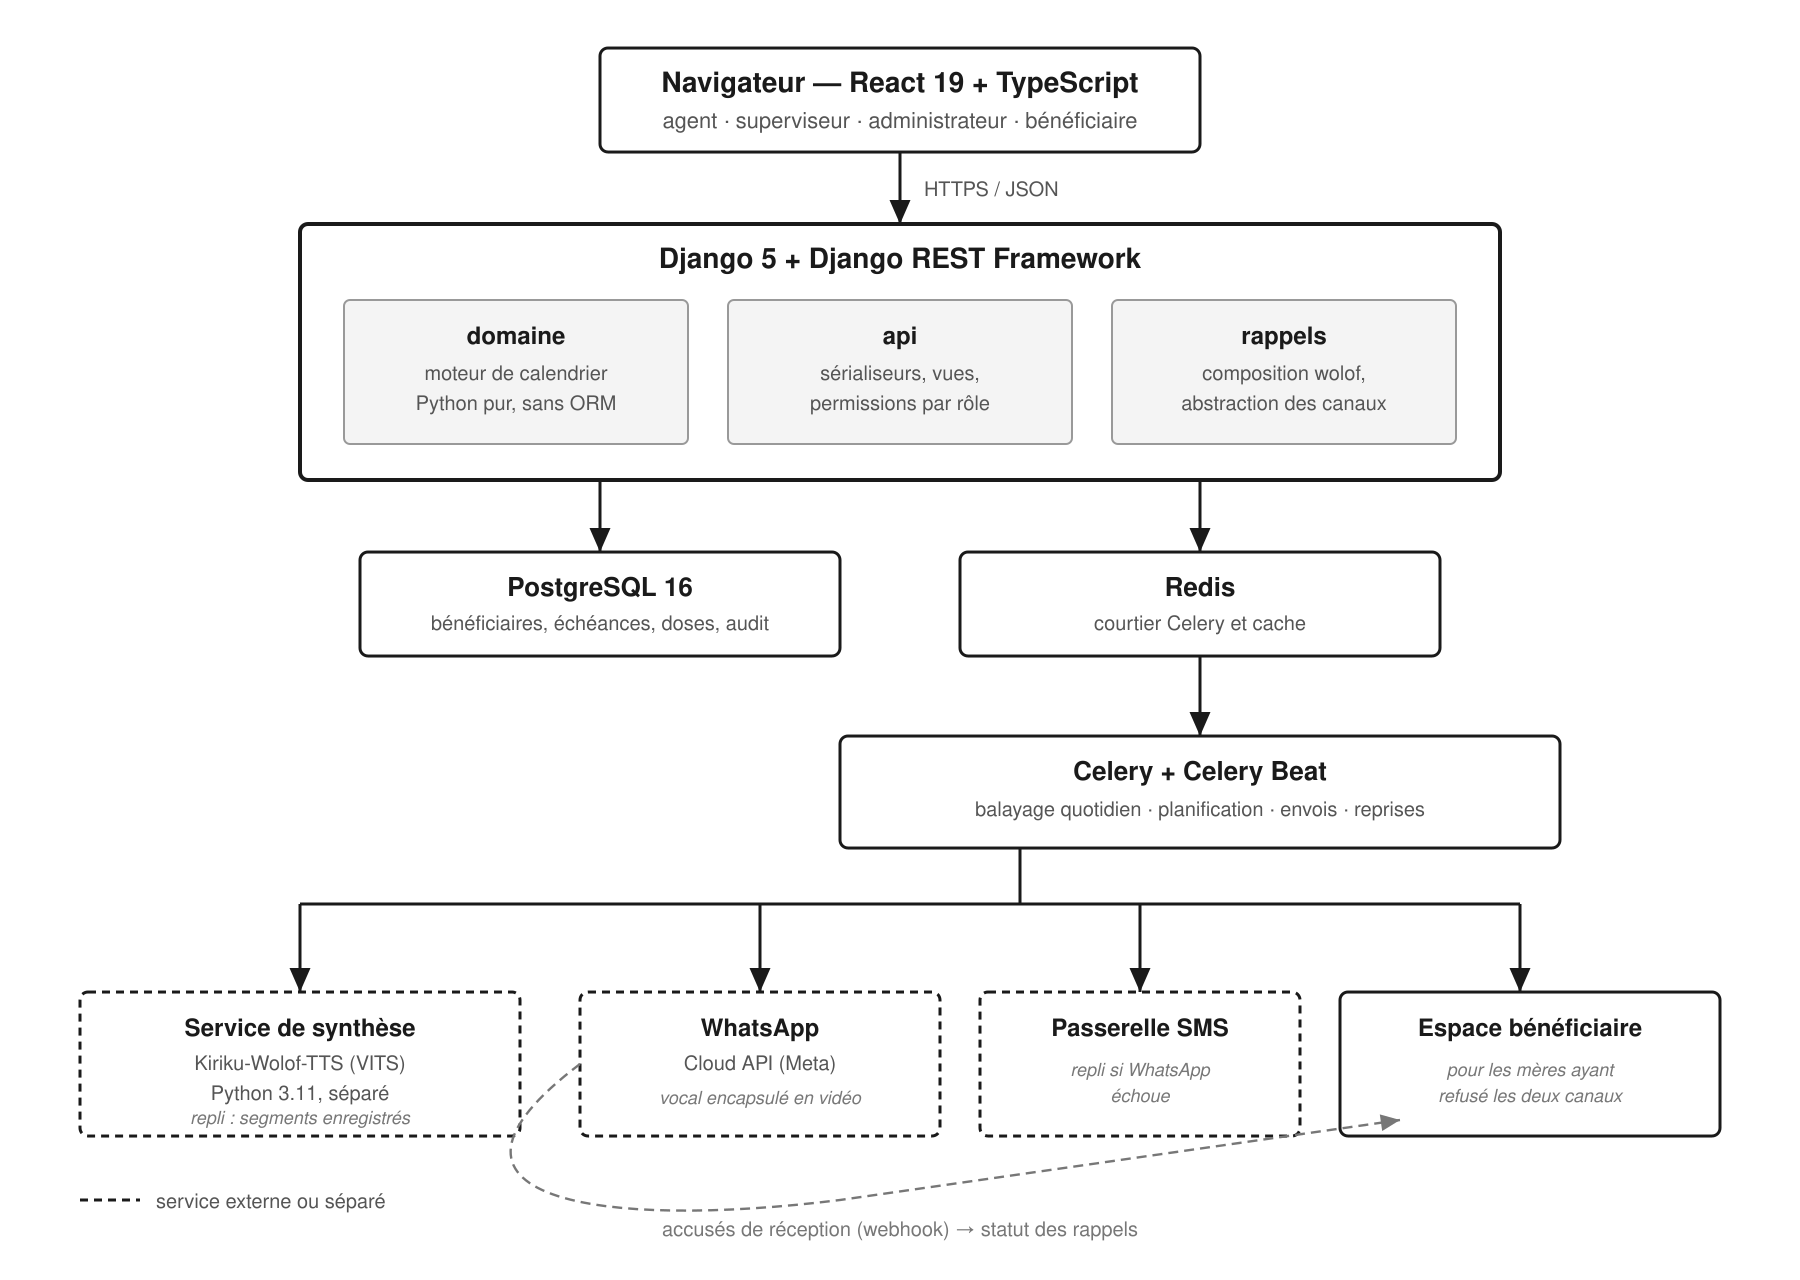
\includegraphics[width=\textwidth]{images/architecture.png}
  \caption{Architecture générale du système}
\end{figure}

Le navigateur dialogue avec Django en HTTPS et JSON. Django porte le moteur
de calendrier, l'API et l'abstraction des canaux de notification. PostgreSQL
conserve les données, Redis sert de courtier à Celery, qui exécute le
balayage quotidien et les envois.

Les messages vocaux passent par un service de synthèse séparé. WhatsApp est
le canal principal, le SMS le repli, et l'application elle-même sert les
mères qui ont refusé les deux.

\section{Diagramme de composants}

\diagramme{06-composants.png}{1.0}{Diagramme de composants}

Le diagramme fait apparaître les interfaces requises et fournies. Deux
points de conception s'y lisent.

\subsection*{L'abstraction des canaux}

Le composant « abstraction des canaux » expose une interface unique
\texttt{Envoi}, implémentée par WhatsApp, le SMS, un canal applicatif et un
canal de simulation. Le code de planification ne connaît aucun de ces
canaux : il demande l'envoi d'un message et reçoit un résultat.

Cette indirection a eu une conséquence heureuse pendant le développement :
l'ensemble de la logique de rappel a pu être écrite et testée avec le canal
de simulation, avant même que le compte WhatsApp ne soit ouvert.

\subsection*{La séparation du service de synthèse}

Le service de synthèse vocale est un composant distinct, appelé en HTTP, et
non une bibliothèque importée. Ce n'est pas un choix esthétique mais une
contrainte subie, documentée dans l'ADR 0009 : le modèle de synthèse wolof
exige Python 3.11, PyTorch et une version ancienne de la bibliothèque
\texttt{transformers}, incompatibles avec le backend qui tourne en Python
3.13 avec Django 5.

L'alternative aurait été de rétrograder l'ensemble du projet. Le coût d'un
service séparé — une pièce de plus à déployer — a paru moindre.

\section{Diagramme de déploiement}

\diagramme{07-deploiement.png}{1.0}{Diagramme de déploiement}

Chaque composant est isolé dans son conteneur. Cette séparation n'est pas
seulement une commodité de développement : elle permet au service de
synthèse d'avoir ses propres dépendances sans contaminer le reste.

\section{Organisation du code}

Le dépôt suit une séparation nette entre le serveur, le client et les
services annexes.

\begin{lstlisting}
suvac/
+-- backend/
|   +-- apps/
|   |   +-- commun/          # bases partagées, données de démonstration
|   |   +-- accounts/        # comptes, postes, audit
|   |   +-- domaine/         # moteur de calendrier (Python pur)
|   |   +-- vaccination/     # référentiel des vaccins et du schéma
|   |   +-- beneficiaires/   # mères, enfants, grossesses, consentements
|   |   +-- suivi/           # échéances et doses
|   |   +-- rappels/         # planification, composition, canaux
|   |   +-- pilotage/        # indicateurs de couverture
|   +-- config/              # configuration Django
+-- frontend/
|   +-- src/
|       +-- api/             # client HTTP et types générés
|       +-- composants/      # bibliothèque d'interface
|       +-- pages/           # écrans
|       +-- etat/            # état applicatif
+-- services/
|   +-- synthese/            # service de synthèse vocale
+-- docs/                    # cahier des charges, ADR, rapport
\end{lstlisting}

Le découpage en applications Django suit les domaines métier et non les
couches techniques. L'application \texttt{domaine} fait exception : elle ne
contient aucun modèle Django, seulement des fonctions de calcul pur.

\section{Contrat d'API typé}

Un point mérite d'être souligné parce qu'il a éliminé une classe entière
d'erreurs.

Django REST Framework génère automatiquement un schéma OpenAPI à partir des
sérialiseurs. Ce schéma est converti en types TypeScript par un générateur,
et ces types sont utilisés par le client. Le contrat est donc vérifié à la
compilation.

\begin{lstlisting}
Sérialiseurs Django  -->  schéma OpenAPI  -->  types TypeScript  -->  client React
\end{lstlisting}

Conséquence concrète : renommer un champ côté serveur fait échouer la
compilation du frontend. L'erreur apparaît à la construction et non à
l'exécution, chez un agent de santé au milieu d'une consultation.

% ====================================================================
% CHAPITRE 5 — RÉALISATION
% ====================================================================
\chapter{Réalisation}

\section{Choix technologiques}

\begin{table}[H]
\centering
\begin{tabularx}{\textwidth}{@{}llX@{}}
\toprule
\textbf{Couche} & \textbf{Technologie} & \textbf{Justification} \\
\midrule
Serveur & Django 5 + DRF & Maturité de l'ORM, administration intégrée,
exigence du module \\
Base & PostgreSQL 16 & Intégrité relationnelle, contraintes de vérification \\
Tâches & Celery + Beat & Planification du balayage et des envois \\
Courtier & Redis & Courtier Celery et cache applicatif \\
Client & React 19 + TypeScript & Exigence du module ; le typage sert
directement la qualité \\
État serveur & TanStack Query & Cache, reprise sur erreur \\
Interface & Tailwind CSS & Jetons de conception propres au projet \\
Synthèse & Kiriku-Wolof-TTS & Seul modèle wolof disponible \\
Conteneurs & Docker Compose & Parité entre environnements \\
Intégration & GitHub Actions & Intégration native au dépôt \\
\bottomrule
\end{tabularx}
\caption{Choix technologiques}
\end{table}

\section{Le moteur de calendrier}

Le moteur est le cœur du système. Il répond à une question : étant donné une
date de naissance et l'historique des doses reçues, quelles échéances
restent à satisfaire, et dans quel état ?

\subsection{Les cinq statuts}

Une échéance peut se trouver dans cinq états.

\begin{description}[leftmargin=2.5cm, style=nextline]
  \item[À venir] La date prévue n'est pas atteinte.
  \item[Due] La date prévue est atteinte ou dépassée de peu ; la dose peut
  être administrée.
  \item[En retard] La date prévue est dépassée significativement, mais la
  dose reste rattrapable.
  \item[Périmée] La date limite est dépassée : la dose n'est plus
  administrable selon le schéma.
  \item[Administrée] Une dose a satisfait l'échéance.
\end{description}

La distinction entre « en retard » et « périmée » n'est pas cosmétique. Elle
détermine si un rappel part encore : relancer une mère pour une dose devenue
inadministrable serait inutile et, pire, lui ferait faire un déplacement pour
rien.

\subsection{Le recalcul après une dose}

Le cas le plus délicat est celui d'une dose administrée en retard. Si un
enfant reçoit sa première dose de pentavalent à dix semaines au lieu de six,
les doses deux et trois ne peuvent pas conserver leurs dates initiales :
l'intervalle minimal de vingt-huit jours ne serait pas respecté.

Le moteur recalcule donc les échéances suivantes à partir de la date
\emph{réelle} d'administration, et non de la date théorique.

\begin{lstlisting}[caption=Principe du recalcul après administration]
Pour chaque échéance suivante de la même série :
    date_minimale = date_dose_precedente + intervalle_min
    date_theorique = date_naissance + age_cible
    nouvelle_date = max(date_minimale, date_theorique)
\end{lstlisting}

Ce comportement fait l'objet de neuf cas de test obligatoires, dérivés
directement du cahier des charges.

\section{La composition des messages wolof}

Le message adressé à la mère n'est pas une traduction mot à mot du libellé
médical. Il a été construit avec un locuteur natif, et les formulations
retenues sont consignées dans un document versionné.

\subsection{Ce que dit le message}

Un rappel comporte quatre éléments : une salutation, la désignation du
bénéficiaire, le vaccin et ce contre quoi il protège, et l'invitation à
venir au poste.

\begin{lstlisting}
Nanga def. Sokhna Ba dafa wara ñakk u ñakk bu lay aar ci juroom i
feebar yu bokkul : diphtérie, tétanos, coqueluche, l'hépatite B ak
infection bu garaw ñu koy woowe Hib tay. Ñëwal ci postu wérgi-yaram bi.
\end{lstlisting}

Le choix d'énoncer les maladies plutôt que le sigle est délibéré. « Votre
enfant doit recevoir le pentavalent » ne dit rien à une mère qui ne connaît
pas ce mot. « Le vaccin qui le protège contre cinq maladies » lui dit
pourquoi se déplacer.

\subsection{Deux garde-fous}

Cette richesse a un coût : la durée. Un message mentionnant trois vaccins
peut atteindre quarante secondes, ce qui est long à écouter.

Deux règles limitent la dérive. Un vaccin n'est jamais répété, même si trois
doses sont en retard. Et au-delà de trois vaccins distincts, le message
résume au lieu d'énumérer.

\section{La production du message vocal}

\subsection{Deux mécanismes}

La production du son a connu une révision en cours de projet, documentée
dans l'ADR 0009.

La conception initiale retenait l'\textbf{assemblage de segments
pré-enregistrés} : une quarantaine de fragments courts — salutations, noms
de vaccins, mois, formules de relance — enregistrés par une voix humaine et
concaténés selon le message à produire. Ce mécanisme offre une voix naturelle
et ne coûte rien à l'exécution.

Son défaut est apparu à l'usage : il ne sait dire que ce qui a été
enregistré. Chaque nouveau poste de santé aurait demandé un enregistrement
supplémentaire, ce qui ne tient pas quand le dispositif s'étend.

La disponibilité d'un modèle de \textbf{synthèse vocale wolof} a permis de
lever cette contrainte. Le modèle Kiriku-Wolof-TTS, d'architecture VITS,
publié par AI Hub Sénégal, prononce le texte composé quel qu'il soit.

Les deux mécanismes coexistent : la synthèse est la voie principale, et
l'assemblage reste le repli quand le service est indisponible.

\subsection{Le coût de la synthèse et sa parade}

La génération coûte entre cinq et vingt secondes par message sur une machine
sans accélérateur graphique. C'est beaucoup trop pour la faire pendant
l'envoi.

Deux parades ont été mises en place. La génération se fait \emph{avant}
l'envoi, dans une étape distincte du balayage. Et les fichiers sont indexés
par l'empreinte du texte, non par le rappel.

Ce second point est ce qui rend la synthèse praticable. Les messages se
répètent beaucoup d'une mère à l'autre : deux enfants devant recevoir le même
vaccin le même jour produisent un texte identique. Un balayage génère donc une
vingtaine de fichiers distincts, et non un par bénéficiaire.

\section{L'encapsulation vidéo}

Un obstacle technique a failli compromettre le projet entier.

WhatsApp n'accepte, en en-tête d'un modèle de message, que du texte, une
image, une vidéo ou un document. \textbf{L'audio n'en fait pas partie.} Or
un message vocal envoyé spontanément, hors de la fenêtre de vingt-quatre
heures ouverte par une réponse de la destinataire, n'est pas réalisable
directement.

La solution retenue consiste à \emph{encapsuler} l'audio dans une vidéo. Un
fichier MP4 est assemblé par \texttt{ffmpeg} à partir d'une image fixe aux
couleurs de l'application et de la piste audio wolof, puis envoyé en en-tête
d'un modèle de catégorie utilitaire.

Le poids reste modeste — de l'ordre de deux cents kilooctets pour vingt
secondes — ce qui compte sur un réseau 2G.

\section{Sécurité}

\subsection{Le cloisonnement par poste}

Un agent n'accède qu'aux bénéficiaires de son poste. Cette règle est
appliquée au niveau de la requête, non de l'affichage : le jeu de résultats
est filtré avant d'être sérialisé, de sorte qu'aucune donnée d'un autre poste
ne transite, même vers un client qui la masquerait.

\subsection{Le mot de passe initial}

Un compte créé par un superviseur reçoit un mot de passe choisi par celui-ci
et transmis oralement. Tant que son détenteur ne l'a pas changé, l'API refuse
toute requête hors du changement lui-même.

Le raisonnement est simple : un mot de passe transmis par un tiers n'est pas
un secret. Sans cette règle, un agent travaillerait des mois avec celui que
son superviseur connaît.

\subsection{L'invalidation des sessions}

Un changement ou une réinitialisation de mot de passe met en liste noire les
jetons de rafraîchissement du compte. Si le mot de passe avait été compromis,
les sessions ouvertes ailleurs tombent.

Une limite est assumée : un jeton d'accès reste valable jusqu'à son
expiration, soit quinze minutes. C'est inhérent aux jetons sans état, et le
prix du choix de ne pas interroger la base à chaque requête.

\subsection{Le journal d'audit}

Chaque acte d'administration — création de compte, réinitialisation,
transfert, fermeture de poste — est journalisé avec son auteur, sa cible et
son horodatage. Le journal est en écriture seule et réservé à
l'administrateur : celui qui est contrôlé ne contrôle pas.

% ====================================================================
% CHAPITRE 6 — QUALITÉ
% ====================================================================
\chapter{Qualité et industrialisation}

\section{Stratégie de tests}

La suite de tests compte 286 tests côté serveur et couvre 87\% du code. Côté
client, la couverture atteint 85,6\%.

\begin{table}[H]
\centering
\begin{tabularx}{\textwidth}{@{}lrX@{}}
\toprule
\textbf{Niveau} & \textbf{Part} & \textbf{Objet} \\
\midrule
Unitaires & $\sim$60\% & Moteur de calendrier, composition des messages,
assemblage audio. Sans base de données. \\
Intégration & $\sim$35\% & API REST, permissions, cloisonnement, webhooks.
Avec base de données. \\
Bout en bout & $\sim$5\% & Parcours critiques de l'interface. \\
\bottomrule
\end{tabularx}
\caption{Répartition des tests}
\end{table}

\subsection{Ce que les tests ont attrapé}

Trois défauts méritent d'être cités, parce qu'ils illustrent ce que les
tests apportent réellement.

\textbf{Le rafraîchissement incomplet.} La fonction de mise à jour des
statuts ne reprenait pas les échéances déjà marquées périmées. Un enfant dont
une dose devenait rattrapable après correction de sa date de naissance restait
bloqué. Le défaut est apparu en écrivant les tests de rappels avec des dates
fixes.

\textbf{Le cloisonnement du webhook.} Un test vérifiant la signature HMAC des
appels entrants a révélé que la vérification était contournable en l'absence
d'en-tête de signature.

\textbf{La vidéo non jointe.} Le service d'envoi composait bien le message et
produisait bien l'audio, mais n'attachait pas la vidéo au message envoyé.
Meta acceptait l'envoi puis rejetait silencieusement le message hors fenêtre
de vingt-quatre heures. Ce défaut n'avait pas été détecté par les tests,
parce que ceux-ci utilisaient le canal de simulation, qui accepte tout — une
limite de la stratégie de test qu'il faut reconnaître.

\section{Intégration continue}

Chaque \emph{pull request} déclenche une chaîne de vérifications :

\begin{enumerate}[leftmargin=1cm]
  \item Formatage du code (Black, oxlint)
  \item Analyse statique (Ruff, TypeScript)
  \item Vérification du typage (mypy)
  \item Contrôle des migrations en attente
  \item Exécution des tests avec seuil de couverture
  \item Analyse des dépendances vulnérables
\end{enumerate}

Un échec bloque la fusion. Cette contrainte a été respectée sans exception :
les quarante-six \emph{pull requests} fusionnées du projet sont toutes
passées par cette chaîne.

\section{Décisions d'architecture}

Neuf décisions structurantes ont été consignées sous forme d'ADR.

\begin{table}[H]
\centering
\small
\begin{tabularx}{\textwidth}{@{}lX@{}}
\toprule
\textbf{ADR} & \textbf{Décision} \\
\midrule
0001 & Langue du code : français pour le domaine, anglais pour la technique \\
0002 & Stratégie de branchement et de fusion \\
0003 & Échéances persistées plutôt que recalculées \\
0004 & Idempotence de la synchronisation \\
0005 & Portée de l'internationalisation \\
0006 & Authentification des bénéficiaires \\
0007 & Authentification et administration du personnel \\
0008 & Traçabilité des actes d'administration \\
0009 & Production des messages vocaux (révisée) \\
\bottomrule
\end{tabularx}
\caption{Décisions d'architecture consignées}
\end{table}

L'ADR 0009 est la seule à avoir été révisée en cours de projet. Sa version
initiale écartait la synthèse vocale au profit des segments enregistrés,
faute de modèle wolof fiable. La disponibilité d'un tel modèle a invalidé la
prémisse, et la décision a été reprise. Conserver la trace de ce
retournement, plutôt que de réécrire l'histoire, fait partie de l'intérêt de
l'exercice.

\section{Volumétrie}

\begin{table}[H]
\centering
\begin{tabular}{@{}lr@{}}
\toprule
\textbf{Indicateur} & \textbf{Valeur} \\
\midrule
Lignes de Python (applications) & $\sim$13 400 \\
Lignes de TypeScript et TSX & $\sim$15 500 \\
Tests serveur & 286 \\
Couverture serveur & 87\% \\
Couverture client & 85,6\% \\
Applications Django & 8 \\
Tables en base & 18 \\
Décisions d'architecture & 9 \\
\bottomrule
\end{tabular}
\caption{Volumétrie du projet}
\end{table}

% ====================================================================
% CHAPITRE 7 — RÉSULTATS
% ====================================================================
\chapter{Résultats}

Ce chapitre présente le système tel qu'il fonctionne, écran par écran.

\section{Authentification}

\capture{01-connexion.png}{1.0}{Écran de connexion}

\section{Le poste de travail de l'agent}

\subsection{La file du jour}

C'est l'écran d'accueil de l'agent, et la réponse à l'objectif OS-2 : savoir
chaque matin qui devrait se présenter.

\capture{02-file-du-jour.png}{1.0}{File du jour — bénéficiaires attendus et
en retard}

Les bénéficiaires sont groupés par urgence. Les doses en retard apparaissent
en premier, puisque ce sont elles qui réclament une action.

\subsection{Le carnet d'un bénéficiaire}

\capture{03-fiche-mere.png}{1.0}{Fiche d'une mère et carnet de ses enfants}

La frise verticale montre le parcours vaccinal complet, du passé administré
aux échéances à venir. C'est la transposition numérique du carnet papier,
avec ce que le papier ne sait pas faire : signaler ce qui est dû.

\subsection{La saisie d'une dose}

\capture{04-saisie-dose.png}{0.8}{Enregistrement d'une dose administrée}

Le formulaire vérifie l'administrabilité avant de permettre
l'enregistrement. Une dose dont l'intervalle minimal n'est pas écoulé est
refusée avec son motif.

\section{Le pilotage du superviseur}

\capture{05-pilotage.png}{1.0}{Tableau de bord du superviseur}

Les indicateurs de couverture sont calculés sur la cohorte réellement
concernée, et non sur l'ensemble des enfants enregistrés. Un enfant de six
semaines ne peut pas faire baisser le taux de couverture du vaccin contre la
rougeole, qui ne lui est dû qu'à neuf mois.

Cette précision est importante : un dénominateur mal choisi produit des
chiffres faux dans le sens rassurant, ce qui est le pire des cas pour un
indicateur de santé publique.

\section{Le journal des rappels}

\capture{06-journal-rappels.png}{1.0}{Journal des rappels émis}

Le journal donne au superviseur ce dont il a besoin pour savoir si ses
messages arrivent : le taux de remise, le taux de lecture, et les motifs
d'échec les plus fréquents.

\capture{07-detail-rappel.png}{0.85}{Détail d'un rappel — texte envoyé et
frise d'acheminement}

Le détail montre le texte wolof exactement tel qu'il a été envoyé. C'est une
exigence de traçabilité : en cas de contestation, on doit pouvoir dire ce que
la mère a reçu.

\section{L'espace de la bénéficiaire}

\capture{08-espace-mere.png}{1.0}{Espace de consultation de la mère}

Cet espace est entièrement en wolof. C'est le seul endroit du système où
l'interface est traduite : le personnel soignant travaille en français, et
traduire son interface aurait été un effort considérable pour un bénéfice
nul.

Cette délimitation est documentée dans l'ADR 0005. Elle illustre une leçon
du projet : l'internationalisation coûte cher, et il vaut mieux la concentrer
là où elle change quelque chose.

\section{L'administration}

\capture{09-personnel.png}{1.0}{Gestion du personnel du poste}

\capture{10-schema-vaccinal.png}{1.0}{Schéma vaccinal en consultation}

Le schéma est consultable mais non modifiable par le superviseur. Une erreur
de saisie recalculerait les calendriers de tous les enfants du poste ; cette
opération relève de l'administrateur.

L'avertissement affiché en tête d'écran mérite un commentaire. Le schéma
utilisé a été reconstitué à partir de sources publiques et n'a pas été validé
par le PEV Sénégal. Plutôt que de masquer cette limite, le système l'affiche.

\capture{11-journal-audit.png}{1.0}{Journal des actes d'administration}

\section{Le rappel reçu}

Voici le résultat qui donne son sens au projet : un rappel vaccinal composé
en wolof, prononcé par synthèse vocale, encapsulé en vidéo, et reçu sur un
téléphone sénégalais.

\capture{12-whatsapp-recu.jpg}{0.40}{Rappel vaccinal reçu sur WhatsApp}

La vignette porte l'identité de l'application. Le corps du message, en
français, nomme l'enfant concerné — il s'adresse à qui sait lire. Le contenu
qui compte est dans la vidéo : le message vocal en wolof.

% ====================================================================
% CHAPITRE 8 — BILAN
% ====================================================================
\chapter{Bilan et perspectives}

\section{Ce qui a été livré}

Les quatre objectifs spécifiques ont été atteints. Le moteur de calendrier
fonctionne et gère les cas difficiles — prématurés, doses en retard,
contre-indications. L'agent dispose de sa file quotidienne. Les rappels
vocaux partent et arrivent. Le superviseur a ses indicateurs.

Le risque le plus sérieux du projet a été levé : rien ne garantissait, au
départ, qu'un message vocal spontané puisse être acheminé par WhatsApp. La
réponse — l'encapsulation vidéo — a été trouvée et vérifiée en conditions
réelles.

\section{Ce qui n'a pas été fait}

\subsection{Le mode hors ligne}

C'est le manque le plus important. Le cahier des charges spécifie sept
exigences relatives au fonctionnement sans connexion, et l'argument de la
connectivité dégradée revient dans la justification du projet.

Ces exigences n'ont pas été réalisées. La pièce la plus difficile est
toutefois en place depuis le premier sprint : la clé d'idempotence qui permet
de rejouer une opération sans la dupliquer. C'est elle qui rend la
synchronisation possible sans créer de doses fantômes.

\subsection{Le code à usage unique}

L'authentification des bénéficiaires repose encore sur un mot de passe
transmis par l'agent. Le remplacement par un code à usage unique envoyé sur
WhatsApp a été conçu mais non livré : il exige un modèle de message d'une
catégorie particulière chez Meta, dont l'obtention n'a pas pu être menée à
terme.

\subsection{L'évaluation de la compréhension}

Les messages wolof ont été validés par un locuteur natif, et le rendu de la
synthèse jugé acceptable à l'écoute. Mais aucune évaluation formelle n'a été
conduite auprès de mères wolophones.

C'est la limite la plus sérieuse du projet, et il faut la nommer : le seul
critère qui compte est qu'une mère de Ndondol comprenne ce qu'elle entend, et
ce critère n'a pas été mesuré.

\section{Ce que le projet a appris}

\subsection{Les contraintes externes dictent la conception}

L'encapsulation vidéo n'est pas une idée élégante : c'est un contournement
imposé par une limitation de Meta. De même, le service de synthèse séparé
n'existe que parce que deux bibliothèques refusent de cohabiter.

Une part importante du travail d'architecture consiste à absorber ce genre de
contraintes sans contaminer le reste du système. L'abstraction des canaux et
la séparation du service de synthèse ont servi exactement à cela.

\subsection{Les tests révèlent ce qu'on ne cherchait pas}

Le défaut du rafraîchissement incomplet a été découvert en écrivant des tests
de rappels, pas des tests de calendrier. Les tests écrits avec des dates fixes
ont exposé une hypothèse implicite sur la date courante.

À l'inverse, la vidéo non jointe est passée au travers, parce que le canal de
simulation acceptait tout. Un test qui simule trop bas ne vérifie rien.

\subsection{Documenter les décisions a une valeur propre}

Les neuf ADR ont servi plusieurs fois à retrouver \emph{pourquoi} un choix
avait été fait, des semaines après. L'ADR 0009, révisée, montre l'intérêt le
plus net : conserver la décision initiale et son renversement donne une
information qu'un document réécrit aurait perdue.

\section{Perspectives}

\begin{description}[leftmargin=1cm, style=nextline]
  \item[Le mode hors ligne] Service worker, base locale et file de
  synchronisation. C'est le chantier prioritaire, et le fondement est en
  place.
  \item[L'évaluation de la compréhension] Faire écouter des messages à des
  mères wolophones sans leur montrer le texte, et mesurer ce qu'elles en
  retiennent.
  \item[La validation du schéma vaccinal] Confronter le référentiel
  reconstitué à une source officielle du PEV.
  \item[Le code à usage unique] Obtenir le modèle d'authentification chez
  Meta et supprimer le mot de passe transmis oralement.
  \item[Le déploiement en conditions réelles] Une expérimentation dans un
  poste de santé volontaire, qui seule permettrait de mesurer l'effet sur les
  doses manquées.
\end{description}

\section{Conclusion}

SUVAC répond à une question simple : comment prévenir une mère qui ne lit pas
que son enfant doit être vacciné.

La réponse technique — un message vocal en wolof acheminé par WhatsApp — a
demandé de résoudre plusieurs obstacles qui n'étaient pas prévisibles au
départ, du refus de l'audio par Meta à l'incompatibilité des bibliothèques de
synthèse. Chacun a été documenté et contourné.

Reste la question qui compte, et qui dépasse le cadre de ce module : est-ce
que cela change quelque chose ? Un système qui fonctionne techniquement n'est
pas un système qui sert. La réponse exigerait une expérimentation sur le
terrain, et c'est la perspective la plus importante de ce travail.

% ====================================================================
% ANNEXES
% ====================================================================
\appendix

\chapter{Installation et vérification}

\section{Prise en main rapide}

\begin{lstlisting}
git clone https://github.com/Fallou236/suvac.git
cd suvac
docker compose up -d

cd backend
python -m venv .venv && source .venv/bin/activate
pip install -r requirements.txt
cp .env.example .env          # renseigner DJANGO_SECRET_KEY
python manage.py migrate
python manage.py charger_schema_pev
python manage.py charger_descriptions
python manage.py charger_donnees_demo --vider
python manage.py runserver

# dans un second terminal
cd frontend && npm install && npm run dev
\end{lstlisting}

L'application est accessible sur \texttt{http://localhost:5173}.

\section{Comptes de démonstration}

Mot de passe commun : \texttt{suvac-demo-2026}

\begin{table}[H]
\centering
\begin{tabularx}{\textwidth}{@{}llX@{}}
\toprule
\textbf{Identifiant} & \textbf{Rôle} & \textbf{À observer} \\
\midrule
\texttt{awa.ndiaye} & Agent, Ndondol & File du jour, saisie d'une dose \\
\texttt{fatou.gueye} & Superviseur, Ndondol & Pilotage, journal des rappels \\
\texttt{omar.diallo} & Superviseur, Ngaparou & Les mêmes écrans, d'autres
chiffres : le cloisonnement \\
\texttt{admin.suvac} & Administrateur & Postes, journal d'audit \\
\texttt{rokhaya.ba} & Bénéficiaire & L'espace de la mère, en wolof \\
\bottomrule
\end{tabularx}
\caption{Comptes du jeu de démonstration}
\end{table}

Toutes les données sont fictives, conformément à ENF-24.

\section{Vérification}

\begin{lstlisting}
cd backend && pytest -q          # 286 tests, 87% de couverture
cd frontend && npm run verifier  # analyse, compilation, tests
\end{lstlisting}

\chapter{Déclencher un balayage}

Pour observer la production des rappels sans attendre l'ordonnanceur :

\begin{lstlisting}
cd backend
python manage.py balayer
\end{lstlisting}

Sans configuration WhatsApp, les rappels partent en simulation et sont
consultables dans le journal avec le compte \texttt{fatou.gueye}.

Pour recevoir un rappel réel, attribuer son numéro à une bénéficiaire :

\begin{lstlisting}
python manage.py charger_donnees_demo --vider --telephone "+221771234567"
python manage.py balayer
\end{lstlisting}

Le numéro doit avoir été déclaré au préalable dans la liste des
destinataires autorisés du compte de test Meta.

\end{document}
